\section{Descrição do problema}

As plataformas são construídas a partir de estruturas modulares, que são
posicionadas com a utilização de guindastes. Esse tipo de estratégia de
construção possibilita a redução do tamanho necessário dos guindastes. A ordem
de grandeza de cada módulo é de dezenas de milhares de toneladas. A
figura \ref{modulos} ilustra a modularidade de uma plataforma e a figura
\ref{fpso_modules} ilustra os módulos em um FPSPO.

 \begin{figure}[h!]
    \centering
    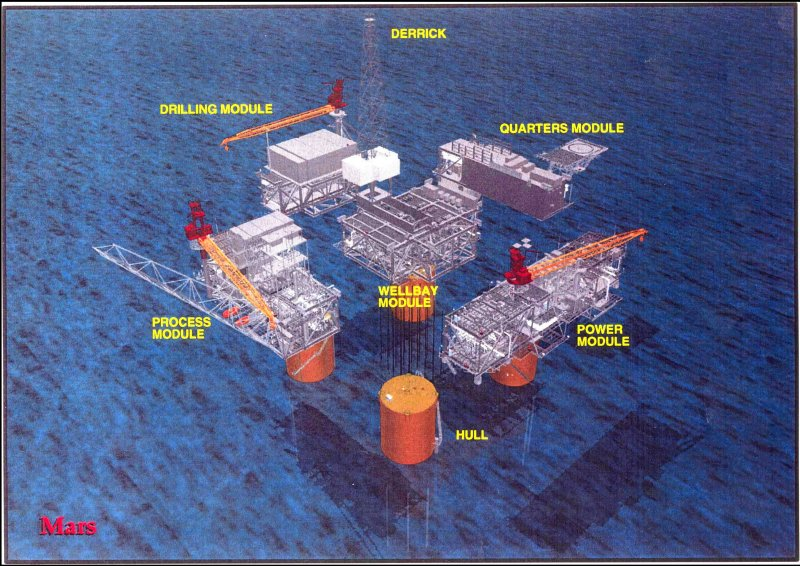
\includegraphics[width=0.9\columnwidth]{figs/mating/modules}
    \caption{Módulos de uma plataforma.}
    \label{modulos}
\end{figure}

\begin{figure}[h!]
    \centering
    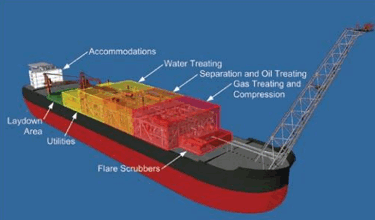
\includegraphics[width=0.9\columnwidth]{figs/mating/fpso_modules}
    \caption{Módulos em um FPSO.}
    \label{fpso_modulos}
\end{figure}


A operação de içamento dos módulos pode ser realizada a partir de guindastes
flutuantes, como no caso da plataforma P-53, o que o que exigia paralisações 
na movimentação de navios na área do Porto Novo, ou por meio de guindastes de grande porte 
fixo em terra, não prejudicando o fluxo hidroviário. Esse tipo de técnica foi
ultizado na plataforma P-63, na qual houve a necessidade da
construção de uma base de concreto de 90 metros de largura por 90 metros de
comprimento, a ser construída no cais.

Por sua vez, a Plataforma P-55 teve todo o seu convés, uma estrutura de 17mil
toneladas, içado no estaleiro a uma altura de 45 metros e acoplado ao casco,
parte inferior da plataforma. Essa técnica nunca havisa sido usada e
possibilitou a construção simultânea dos dois módulos. A figura\ref{P55} ilustra
o alinhamento entre os dois módulos sendo realizado.

\href{http://www.offshoreenergytoday.com/brazils-petrobras-completes-deck-mating-on-p-55-platform/}{P-55\textit{Deck
Mating}}

\begin{figure}[h!]
    \centering
    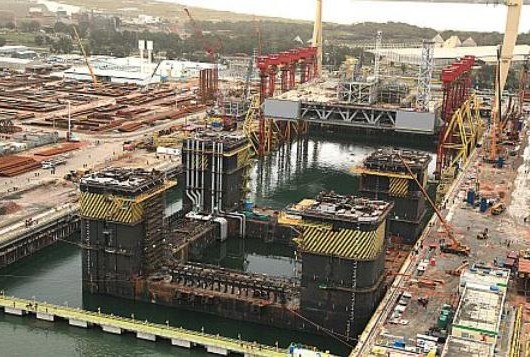
\includegraphics[width=0.9\columnwidth]{figs/mating/P55}
    \caption{Alinhamento da plataforma P-55.}
    \label{P55}
\end{figure} 


